% !TEX TS-program = pdflatex
% !TEX encoding = UTF-8 Unicode

% This is a simple template for a LaTeX document using the "article" class.
% See "book", "report", "letter" for other types of document.

\documentclass[10pt]{article} % use larger type; default would be 10pt
\linespread{1.3}
\usepackage{polski}
\usepackage[utf8]{inputenc} % set input encoding (not needed with XeLaTeX)
\usepackage[letterpaper, portrait, margin=2.5cm]{geometry}

%\usepackage{helvet}
\usepackage{indentfirst}
%\renewcommand{\familydefault}{\sfdefault}
%%% Examples of Article customizations
% These packages are optional, depending whether you want the features they provide.
% See the LaTeX Companion or other references for full information.

%%% PAGE DIMENSIONS
\usepackage{geometry} % to change the page dimensions
\geometry{a4paper} % or letterpaper (US) or a5paper or....
% \geometry{margin=2in} % for example, change the margins to 2 inches all round
% \geometry{landscape} % set up the page for landscape
%   read geometry.pdf for detailed page layout information

\usepackage{graphicx} % support the \includegraphics command and options

% \usepackage[parfill]{parskip} % Activate to begin paragraphs with an empty line rather than an indent

%%% PACKAGES
\usepackage{booktabs} % for much better looking tables
\usepackage{array} % for better arrays (eg matrices) in maths
\usepackage{paralist} % very flexible & customisable lists (eg. enumerate/itemize, etc.)
\usepackage{verbatim} % adds environment for commenting out blocks of text & for better verbatim
\usepackage{subfig} % make it possible to include more than one captioned figure/table in a single float
\usepackage{multicol}
\usepackage{amsmath}
\usepackage{amssymb}
\usepackage{bm}
\usepackage{svg}
\usepackage{amsthm}
\usepackage{ bbold }

%\usepackage{braket}
% These packages are all incorporated in the memoir class to one degree or another...

%%% HEADERS & FOOTERS
\usepackage{fancyhdr} % This should be set AFTER setting up the page geometry
\pagestyle{fancy} % options: empty , plain , fancy
\renewcommand{\headrulewidth}{0pt} % customise the layout...
\lhead{}\chead{}\rhead{}
\lfoot{}\cfoot{\thepage}\rfoot{}
	
%%% SECTION TITLE APPEARANCE
\usepackage{sectsty}
\allsectionsfont{\sffamily\mdseries\upshape} % (See the fntguide.pdf for font help)
% (This matches ConTeXt defaults)

%%% ToC (table of contents) APPEARANCE
\usepackage[nottoc,notlof,notlot]{tocbibind} % Put the bibliography in the ToC
\usepackage[titles,subfigure]{tocloft} % Alter the style of the Table of Contents
\renewcommand{\cftsecfont}{\rmfamily\mdseries\upshape}
\renewcommand{\cftsecpagefont}{\rmfamily\mdseries\upshape} % No bold!

%%% END Article customizations

%%% Math ops %%%
\DeclareMathOperator{\Trs}{Tr}

%%% END

%%% Extra commands %%%
\newcommand{\Mats}[1]{\mathcal{L}(#1)}
\newcommand{\Hx}[1]{\mathcal{H}^{#1}}
\newcommand{\LHx}[1]{\Mats{\Hx{#1}}}
\newcommand{\HAi}{\Hx{A_1}}
\newcommand{\LHAi}{\Mats{\HAi}}
\newcommand{\MXi}[3]{\mathcal{M}^{#1}_{#2}(#3)}
\newcommand{\MXin}[2]{\mathcal{M}^{#1}_{#2}}
\newcommand{\MAin}[0]{\MXin{A}{i}}
\newcommand{\MAi}[1]{\MXi{A}{i}{#1}}
\newcommand{\MAir}{\MAi{\rho}}
\newcommand{\Idx}[1]{\mathbb{1}^{#1}}
\newcommand{\Tr}[1]{\Trs(#1)}
\newcommand{\Pro}[1]{\Pr(#1)}
\newcommand{\Prt}[2]{\Pr(#1, #2)}
\newcommand{\Ket}[1]{|#1\rangle}
\newcommand{\Bra}[1]{\langle#1|}
\newcommand{\BBra}[1]{\langle\langle#1|}
\newcommand{\KKet}[1]{|#1\rangle\rangle}
\newcommand{\Braket}[1]{\langle#1\rangle}
\newcommand{\CP}{\textit{completely positive}}
\newcommand{\TP}{\textit{trace preserving}}
\newcommand{\CPTP}{\textit{completely posite trace preserving}}
\newcommand{\WAll}{W^{A_1A_2B_1B_2}}
\newcommand{\MA}{M^{A_1A_2}}
\newcommand{\MB}{M^{B_1B_2}}
\newcommand{\mai}[1]{\MA_{#1}}
\newcommand{\mbi}[1]{\MB_{#1}}
\newcommand{\KP}{\Ket{\psi}}
\newcommand{\BP}{\Bra{\psi}}
\newcommand{\X}{\mathbb{X}}
\newcommand{\Y}{\mathbb{Y}}
\newcommand{\Z}{\mathbb{Z}}
\newcommand{\I}{\mathbb{1}}
\newcommand{\IO}{\mathbb{1}^\circ}

%%% END

%%% The "real" document content comes below...

\title{Przyczynowe więzy na strukturę korelacji w formalizmie kwantowym}
\author{Piotr Krasuń}
%\date{} % Activate to display a given date or no date (if empty),
         % otherwise the current date is printed 
\setlength{\parindent}{1.25cm}
\begin{document}
\maketitle
\tableofcontents
\newpage
\listoffigures
\listoftables
\newpage
%\begin{multicols*}{2}
\section{Wstęp}
%%%%
\subsection{Historia}
Mechanika kwantowa od samego początku jej badania budziła wiele kontrowersji. Od samego początku wiele osób miało problem z zaakceptowaniem faktu, iż
na fundamentalnym poziomie rzeczywistość nie jest deterministyczna, jak nam się wydawało. Losowa natura tej teorii, jak i wiele "dziwnych" cech mechaniki kwantowej była początkowo trudna do zaakceptowania. Rok po opublikowaniu pracy Schrödingera, Einstein w swojej pracy zamieścił zdanie, które kierunkowało badania w tamtym czasie, zaś dziś w raz z innymi popularnymi "powiedzonkami" kwantowymi zakorzeniony w kulturze, a mianowicie, że "Bóg nie gra w kości", która później okazała się być nieprawdziwa - przynajmniej nie w takim stopniu w jakim autor by sobie życzył. Sam formalizm doczekał się wielu interpretacji często bardziej filozoficznych. Dzisiaj najpopularniejszymi jest interpretacja Kopenhaska, teoria wielu światów, czy idei inkorpującej kwantowej grawitacje w mechanizmie pomiaru. Mimo tego jest to bardzo matematycznie elegancka teoria, którą można nazwać jednym z największych osiągnięć współczesnej fizyki. Wielokrotnie jej "dziwne" przewidywania zostały potwierdzane eksperymentalnie z wręcz idealna dokładnością (w przeciwieństwie do np. stałej kosmologicznej, która niedokładność przekracza wiele dziesiątek rzędu wielkości). 
\subsection{Podstawowe informacje}
Przechodząc do bardziej konkretnych rzeczy; systemy w mechanice kwantowej opisuję się jako elementy przestrzeni Hilberta $\psi \in \Hx{}$, a tak zwane obserwable samosprzężone operatorów $A \in \LHx{}$, które opisują nam pomiary, jakie możemy wykonać na danym systemie. W przypadku skończenie wymiarowym, bądź policzalnym możemy powiedzieć, że $\Hx{A} = \mathcal{C}^N$ i
obserwable są po prostu macierzami hermitowskimi odpowiedniego wymiaru. Przez znak równa się rozumiemy przestrzeń Hilberta zbudowana na tym zbiorze z odpowiednimi działaniami. Dosyć standardowym i wygodnym jest wykorzystywanie tak zwanej notacji Diraca a mianowicie przedstawianie $\psi = \Ket{\psi}$ i $\psi^\dag = \Bra{\psi}$
\begin{align}
\psi = 
\begin{pmatrix}
a_1\\a_2\\a_3
\end{pmatrix}
:= \Ket{\psi}
\quad & \quad\psi^\dag = 
\begin{pmatrix}
a_1^*~a_2^*~a_3^*
\end{pmatrix}
:= \Bra{\psi}
\end{align}
\begin{figure}[th]
\centering
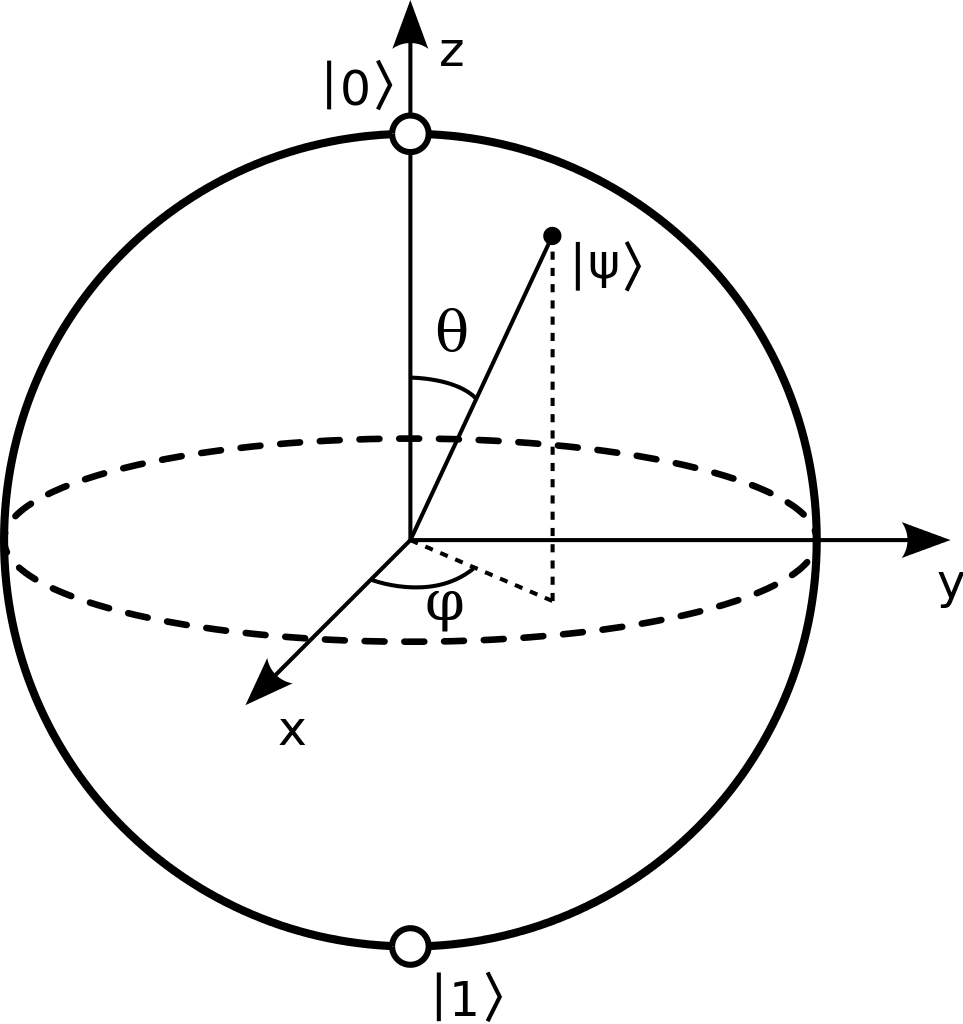
\includegraphics[width=0.20\textwidth]{obrazki/Bloch_sphere}
\caption{Sfera Blocha. Punkty na tej sferze opisują wszystkie możliwe stany $\KP$.}
\label{fig:bloch}
\end{figure}
Wygodnie narzucić warunek normalizacji stanów, a mianowicie $\Bra{\psi}\Ket{\psi} := \Braket{\psi|\psi} = 1$, wtedy wartość oczekiwaną obserwabli w danym stanie $\Ket{\psi}$ oblicza się tak $\Braket{A} := \Bra{\psi}A\Ket{\psi}$. Zauważmy, że skoro obserwable opisywane są przez macierze hermitowskie, można 
skorzystać z twierdzenia spektralnego i zapisać $A = \sum_i^N \lambda_i \Ket{i}$, gdzie $\lambda_i$ opisuje i-tą wartość własna zaś $\Ket{i}$ to i-ty wektor własny, który dobrano tak, że $\Braket{i|j} = \delta_{ij}$, $\{\Ket{i}\}$ tworzy ortonormalna bazę w $\Hx{}$. Jednym z postulatów mechaniki kwantowej jest tzw. postulat pomiaru von Neumanna. Mówi on, że wykonując pomiar obserwabla A system w stanie $\Ket{\psi}$ otrzymamy wartość $\lambda_i$ odpowiadająca wektorowi własnemu $\Ket{i}$ zapada się w stan $\Ket{i}$. Można zapisać go w następujący sposób opisujący warunkową ewolucję po pomiarze
\begin{equation}
\label{eq:cond_ev}
\Ket{\psi} \mapsto \frac{\Pi_i\Ket{i}}{\sqrt{\Bra{\psi}\Pi_i \Ket{\psi}}},
\end{equation}
gdzie $\Pi_i$ jest projektorem odpowiadającym $\Ket{i}\Bra{i}$. Zapisująć $\KP = \sum^N_i a_i \Ket{i}, \sum^N_i |a_i|^2=1$ prawdopodobieństwo zaobserwowania wyniku $\lambda_i$ jest równe $|a_i|^2$, lub równoważnie
\begin{equation}
\Pro{\lambda_i} = \BP \Pi_i \KP,
\end{equation}
co znane jest jako reguła Borna. Fakt, że obserwable są opisywane przez macierze Hermitowskie zapewnia, że $\sum^N_i \Ket{i}\Bra{i} = \mathbb{1}$, co dalej implikuje, że $\sum^N_i \Pro{\lambda_i} = \sum^N_i \BP \Pi_i \KP = \BP \sum^N_i \Pi_i \KP = \Braket{\psi | \psi} = 1$
Stan całego systemu składającego się z pewnej ilości systemów opisuje element z
\begin{equation}
\Hx{AB\dots} = \Hx{A} \otimes \Hx{B} \otimes \dots,
\end{equation}
gdzie $\otimes$ to iloczyn tensorowy. W raz z wzrostem systemów składających się na system ilość wektorów bazowych rośnie ekspotencjalnie, co jest fundacją tzw. "kwantowego przyśpieszenia", które pozwala heurystycznie/przybliżenie rozwiązać na komputerach kwantowych problemy niektóre klasyczne problemy z ekspotencjalnym przyśpieszeniem
np. faktoryzacja liczb, rozwiązywanie układów liniowych czy odpowiednio sformułowane problemy uczenia maszynowego.
Ważną rzeczą do zaobserwowania jest fakt, że istnieją takie systemy, które nie można zapisać, jako iloczyn stanów w poszczególnych podsystemach. Klasycznym przykładem tego jest
\begin{gather*}
\Hx{AB} = \mathcal{C}^2 \otimes \mathcal{C}^2 \\
\KP = \Ket{1}_A \otimes \Ket{1}_B + \Ket{0}_A \otimes \Ket{0}_B := \Ket{1}\Ket{1} + \Ket{0}\Ket{0} := \Ket{11} + \Ket{00} \\
a_0\Ket{0} + a_1\Ket{1} \otimes b_0\Ket{0} + b_1\Ket{1} = a_0b_0 \Ket{00} + a_0b_1\Ket{01} + a_1b_0\Ket{10} + a_1b_1\Ket{11} \\
a_0b_1 = 0\implies a_0 = 0\vee b_1 = 0 \\
a_1b_0 = 0\implies a_1 = 0\vee b_0 = 0 \\
\text{Powyższe implikują, że } a_0b_0 \neq 1 \vee a_1b_1 \neq 1.
\end{gather*} Takie systemy, które nie da się zapisać w postaci $\Ket{\Psi} = \Ket{\psi}_A \otimes \Ket{\phi}_B$ nazywa się splątanymi. Splątanie kwantowe jest zasobem, które znalazło zastosowanie w wielu nowatorskich aplikacjach, jak np. kryptografia kwantowa, certyfikowana losowość, teleportacja kwantowa czy wcześniej przytoczone "kwantowe przyśpieszenie".
Często w rozważaniach ogranicza się do skończonych przestrzeni Hilberta o wybranych rozmiarach. Najmniejszą i niepodzielnym jednostką informacji jest kubit ($\Hx{} = \mathcal{C}^2$), fizycznie reprezentuje on np. cząstkę ze spinem-$\frac{1}{2}$ (elektron), polaryzację fotonu. W wielu dziedzinach informatyki kwantowej ogranicza się praktycznie wyłącznie do analizy systemów złożonych z kubitów ze względu
na pewną prostotę i wygodę analizy takich systemów. Ciekawą interpretacją kubitów prezentuje Sferta Blocha (\ref{rys. fig:bloch}). Punkty na tej sferze opisują wszystkie prawidłowe znormalizowane $\KP \in \mathcal{C}^2$.
Okazuje się jednak, że niewystarczający do opisu zespołów statystycznych (system znajduje się w jakimś z $\Ket{\psi_i}$ stanów z prawdopodobieństwem $p_i$) wynikający z braku pełnej wiedzy o systemie, bądź sposobie jego przygotowania. Do opisu takich sytuacji korzysta się z macierzy gęstości, definiowanych następująco
\begin{gather}
\rho = \KP \BP \\
\Braket{A} = \Tr{A\rho} \\
\Pro{\lambda_i} = \Tr{\Pi_i \rho}\\
\rho \mapsto \frac{\Pi_i\rho\Pi_i}{\Trs(\Pi_i\rho)}
\end{gather}
Prócz warunkowej ewolucji podczas pomiaru, systemu kwantowe podlegają również ewolucji czasowej. W obrazie Schrödingera ewoluują stany. Wygłada to następująco
\begin{gather}
U(t)\Ket{\psi(0)} = \Ket{\psi(t)} \\
U(t)^\dag\Ket{\psi(t)} = \Ket{\psi(0)}
\end{gather}
Zaś w obrazie Heisenberga ewoluują obserwable
\begin{gather}
A(t) = U^\dag A(0)U
\end{gather}
gdzie $U(t)$ jest pewnym unitarnym operator ($U^\dag U = \mathbb{1}$) działającym na $\Hx{}$. Pomiar rzutujący nie jest jedynym pomiarem, który można wykonać. Najogólniejszym pomiarem, który można wykonać w mechanice kwantowej jest \textit{positive valued measurement} (POVM). Opisywany jest on przez
zbiór takich operatorów $\{E_i\}$, że $E_i > 0,~\sum_i E_i = \mathbb{1}$. Poprzednie reguły przechodzą w
\begin{gather}
\Pro{x_i} = \Bra{\psi} E_i \Ket{\psi}\\
\Pro{x_i} = \Tr{E_i \rho} \\
E_i = \sum_j = A^\dag_{ij}A_{ij} \\ 
\rho \mapsto \frac{\sum_j A_{ij} \rho A^\dag_{ij}}{\Tr{\sum_j A_{ij} \rho A^\dag_{ij}}},
\end{gather} pomiary takie realizuje się korzystając z \textit{ancilli} (pomocniczy system), ewoluując złożony system odpowiednio dobranym operatorem unitarnym, następnie dokonując pomiaru rzutującego na \textit{ancilli} i po odnotowaniu wyniku odrzuceniu jej.
% tutaj moze przyklad
Ważnym narzędziem w formalizmie kwantowym są tak zwane kanały kwantowe \textit{quantum channel} opisują one fizyczne połączenia, ich działania na fizyczny system. Klasycznym analogiem może być np. linia telefoniczna czy światłowód transmituje internet. 
Przykładem fizycznej implementacji może znów być światłowód, który transmituje fotony, opisywany jako kubit. 
Kanały kwantowe opisują mapy $\mathcal{M}: \mathcal{L}(\Hx{A}) \to \mathcal{L}{\Hx{B}}$ mapujące liniowe operatory w przestrzeni wejściowej na liniowe operatory w przestrzeni wyjściowej, gdzie $\mathcal{M}$ jest \textit{completely positive} (CP)\footnote
{
Mapę $\phi: A \to B$ nazywa się nieujemną gdy $\phi(a) \geq 0 \forall a\geq 0 \in A$. Nazywama się ją CP gdy $\phi \otimes \mathcal{I}_n$ również jest nieujemna $\forall n \in \mathcal{N}$
}, $\mathcal{M}(\mathbb{1}) = \mathbb{1}$. Najogólniej kanały idealne czyli takie z których możemy otrzymać pełna informację o przychodzącym systemie opisuje się $\mathcal{M}(\rho) = U^* \rho U$, gdzie U jest pewną macierzą unitarną. W rzeczywistych sytuacjach jednakże nie da się uniknąć
oddziaływania z otoczeniem, który posiada dodatkowe niemierzalne stopnie swobody takie zaszumione kanały opisuje ogólnie $\mathcal{M}(\rho) = \Trs_{otoczenie}(U* \rho \otimes \rho_0 U)$, gdzie $\Trs_{otoczenie}$ opisuje operację śladu częściowego po stopniach swobody otoczenia, zaś operator unitarny U
opisuję ewolucję czasową systemu i otoczenia, zaś $\rho_0$ jest stanem początkowym otoczenia \cite{fund}. Jasnym jest, że posiadając wyłącznie wiedzę na temat systemu $\rho$ nie jesteśmy wstanie w ogólności odtworzyć informacji wysłanych.
Typowym przykładem takiego zaszumionego kanału może być kanał depolaryzujący, który z prawdopodobieństwem $\eta$ idealnie transmituje system zaś $1-\eta$ prawdopodobieństwa depolaryzacji, $\mathcal{M}(\rho) = \eta\rho+(1-\rho)\I$. Najogólniejszym modelem kanałów kwantowych jest tzw.
\textit{quantum channel with memeory} (kwantowy kanał z pamięcią) opisany np. w \cite{memory}.

%%%%
\section{Macierz Procesu}
\label{macierz_procesu}
Jednym z podejść do eksploracji korelacji nie zachowujących przyczynowego porządku jest rozwinięty w \cite{process_matrix} formalizm macierzy procesu.
Ewidentną zaletą tego podejścia jest zgodność z mechanika kwantową na poziomie lokalnych eksperymentów. Jest to nijakie rozszerzenie i enkapsulacja idei POVM i reguły Borna. Podejście te porzuca założenie globalnej struktury czasoprzestrzeni. W celu zachowania zgodności z mechaniką kwantową na poziomie lokalnym opiera się na następujących założeniu, że operacje wykonywane przez poszczególną stronę są opisywane przez mechanikę kwantową w standardowym przyczynowym sformułowaniu, które można opisywać przy pomocy zbioru \textit{quantum instruments} \cite{quantum_instrument} z wejściową przestrzenią Hilberta $\mathcal{H}^{A_1}$ i przestrzenią wyjściową  $\mathcal{H}^{A_2}$. Najogólniej można je realizować przy pomocy zadziałania unitarną transformacją na system wejściowy i \textit{ancilla}, następnie wykonanie rzutującego pomiaru na części systemu pozostawiając pozostała część systemu jako wyjście. Alicja wykorzystując dany instrument otrzymuje jeden z możliwych wyników $x_i$, który indukuję transformację $\mathcal{M}^A_i$ z wejścia na wyjście. Transformacja ta odpowiada \CP~(CP) \TP~mapie
\begin{equation}
\mathcal{M}^A_i : \mathcal{L}(\mathcal{H}^{A_1}) \mapsto \mathcal{L}(\mathcal{H}^{A_2})
\end{equation}
gdzie $\LHx{X}$ jest przestrzenią macierzy na $\Hx{X}$, której wymiar to $d_X$. Jej działanie na macierz gęstości $\rho$ opisuje następująca formuła
\begin{equation}
\label{yolo}
\MAi{\rho} = \sum^m_{j=1} E_{ij} ^\dag \rho E_{ij}
\end{equation}
gdzie macierze $E_{ij}$ spełniają następujące własności 
\begin{gather}
\sum^m_{i=0} E_{ij}^\dag E_{ij} \leq \Idx{A_1} \\
\label{eq:id_proj} 
\sum^n_{i=0} \sum^m_{j=0} E_{ij}^\dag E_{ij} = \Idx{A_1}
\end{gather}
Prawdopodobieństwo zaobserwowania wyniku realizowanego przez mapę $\MAin$ to
\begin{equation}
\Pro{\MAin} = \Tr{\MAir}
\end{equation}
Widzimy od razu, że równanie \eqref{eq:id_proj} narzuca, by możliwość zaobserwowania dowolnego wyniku była równa 1.
W przypadku, gdy mamy do czynienia z więcej niż jedną stroną \textit{procesem} będziemy nazywać listę $\Pr(\MXin{A}{i}, \MXin{B}{j}, \dots)$ dla wszystkich możliwych lokalnych wyników. Dalej w tym rozdziale będzie opisywany wyłącznie przypadek dwustronny, jednakże rozszerzenie formalizmu na przypadek wielostronny jest trywialny. Wygodnym sposobem przedstawiania map $\MAin$ jest izomorfizm Choi-Jamiołkowsky (CJ) \cite{cj_iso1, cj_iso2}. Macierz CJ $M^{A_1A_2}_i \in \Mats{\Hx{A_1} \otimes \Hx{A_2}} \geq 0$ jest zdefiniowana jako
\begin{gather}
\label{eq:cj_iso}
M^{A_1A_2}_i := [\mathcal{I} \otimes \MAi{ \KKet{I} \BBra{I}}]^T, \\
\KKet{I} = \sum^{d_{A_1}}_{i=1} \Ket{ii},
\end{gather}
gdzie $\{\Ket{j}\}^{d_{A_1}}$ tworzy ortonormalna bazę w $\HAi$. Korzystając z tego przejścia można zapisać prawdopodobieństwo dwóch rezultatów, jako 
\begin{equation}
\label{eq:cj_prob}
\Prt{\MAin}{\MXin{B}{j}} = \Tr{\WAll(M^{A_1A_2}_i \otimes M^{B_1B_2}_j)}.
\end{equation}
Macierz $W$ w $\Mats{\Hx{A_1} \otimes \Hx{A_2} \otimes \Hx{B_1} \otimes \Hx{B_2}}$ nazywa się \textit{process matrix} (macierzą procesu).
W celu generowania prawidłowego prawdopodobieństwa narzuca się dodatkowe warunki na $W$
\begin{gather}
\label{eq:non_neg}
\WAll \geq 0. \\
\label{eq:sums_to_id1}
\Trs
\left[
\WAll
\left(
M^{A_1A_2} \otimes M^{B_1B_2}
\right)
\right]=1.\\
\label{eq:sums_to_id2}
\forall M^{A_1A_2}, M^{B_1B_2} \geq 0, \Trs_{A_2} \MA = \mathbb{1}^{A_1}, \Trs_{B_2} \MB = \mathbb{1}^{B_1},
\end{gather}
gdzie $\MA = \sum_i \mai{i}$. Warunek \eqref{eq:non_neg} zapewnia, że prawdopodobieństwa nie będą ujemne, a \eqref{eq:sums_to_id1} i  \eqref{eq:sums_to_id2} pewność zaobserwowania dowolnej pary map. 
%tutej moze macierz gestosci
\begin{figure}[t]
\centering

\begin{tabular}{|c|c|c|c|}
\hline
Przyczynowy porządek & Stany & Kanały & Kanały z pamięcią \\
\hline
$A \npreceq B $ & $A_1, B_1, A_1B_1$ & $A_1B_2$ & $A_1B_1B_2$\\
\hline
$B \npreceq A $ & $A_1, B_1, A_1B_1$ & $A_2B_1$ & $A_1A_2B_1$\\ 
\hline
& 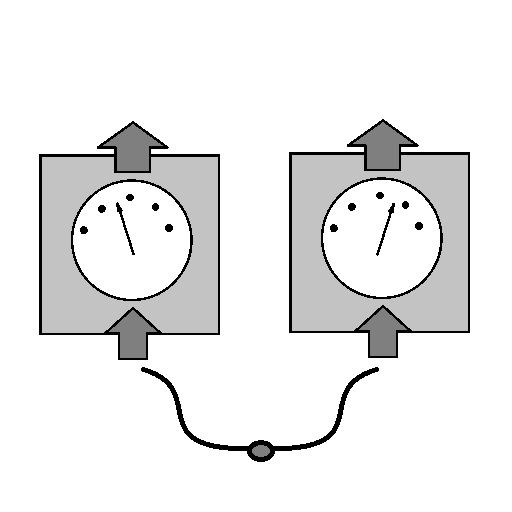
\includegraphics[width=0.2\textwidth]{obrazki/states} & 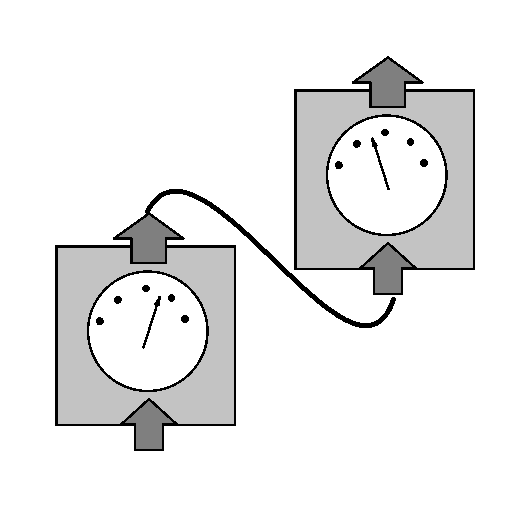
\includegraphics[width=0.2\textwidth]{obrazki/channel}& 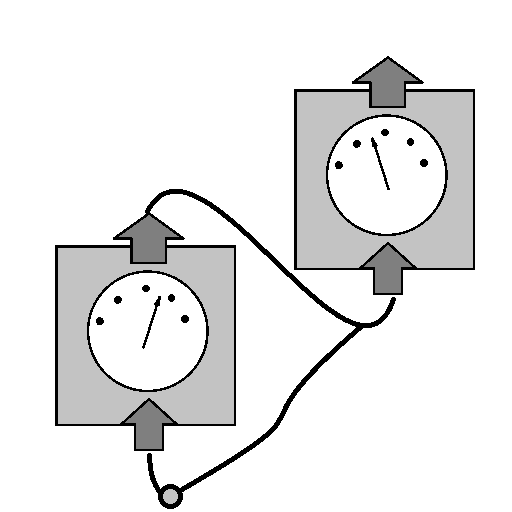
\includegraphics[width=0.2\textwidth]{obrazki/channel_with_memory}\\
\hline
\end{tabular}
\caption{Wyrażenia zgodne z formalizmem i ich proponowana graficzna interpretacja}
\label{fig:configs}
\end{figure}
Baza Hilberta-Schmidta dla $\LHx{X}$ dane jest przez zbiór macierzy $\{\sigma^X_\mu\}^{d^2_X-1}_{\mu=0},$ gdzie $\sigma^X_0 = \mathbb{1}, \Tr{\sigma^X_\mu\sigma^X_\nu}=d_x\delta_{\mu\nu}, \Tr{\sigma^X_{\mu>0}}=0.$ Ogólny element przestrzeni $\Mats{\Hx{A_1}\otimes\Hx{A_2}\otimes\Hx{B_1}\otimes\Hx{B_2}}$ można zapisać, jako
\begin{gather}
\WAll = \sum_{\mu\nu\lambda\gamma}= w_{\mu\nu\lambda\gamma} \sigma_\mu^{A_1}\otimes\sigma_\nu^{A_2}\otimes\sigma_\lambda^{B_1}\otimes\sigma_\gamma^{B_2} \\
w_{\mu\nu\lambda\gamma} \in \mathcal{C} \nonumber.
\end{gather}
Wyrażenia zawierające wyłącznie wyrazy $\sigma^{A_1}_i \otimes \mathbb{1}^{reszta},~(i > 0)$ nazywa się wyrażeniami typu $A_1$, wyrażenia zawierające  $\sigma^{A_1}_i \otimes \sigma^{A_2}_j \otimes \mathbb{1}^{reszta},~(i, j > 0)$ nazywa się wyrażeniami typu $A_1A_2$ etc.
Na rysunku \ref{fig:configs} przedstawiono wyrażenia spełniające \eqref{eq:non_neg} i \eqref{eq:sums_to_id1}. Najogólniejsza macierz procesu zgodna z założeniami to
\begin{gather}
\WAll = \frac{1}{d_{A_1}d_{B_1}}(\mathbb{1} +\sigma^{B \preceq A} + \sigma^{A \preceq B} + \sigma^{A \npreceq \nsucceq B}) \\
\sigma^{A \preceq B} := \sum_{ij>0} a_{ij} \sigma^{A_1}_i \sigma^{B_2}_j + \sum_{ijk>0} b_{ijk} \sigma^{A_1}_i \sigma^{B_1}_j \sigma^{B_2}_k \\
\sigma^{B \preceq A} := \sum_{ij>0} c_{ij} \sigma^{A_2}_i \sigma^{B_1}_j + \sum_{ijk>0} d_{ijk} \sigma^{A_1}_i \sigma^{A_2}_j \sigma^{B_1}_k \\
 \sigma^{A \npreceq \nsucceq B} := \sum_{i>0} e_i  \sigma^{A_1} + \sum_{i>0} f_i  \sigma^{B_1} + \sum_{ij>0} h_{ij} \sigma^{A_1}_i \sigma^{B_1}_j \\
 \forall_{ij} a_{ij}, b_{ij}, c_{ij}, d_{ij}, e_{ij}, f_{ij}, g_{ij}, h_{ij} \in \mathcal{R} \nonumber.
\end{gather}
\section{Przyczynowa separowalność i przyczynowe nierówności}
Macierzami procesu \textit{casually separable} (przyczynowo separowalnymi) nazywa się takie macierz, które można zapisać jako wypukła kombinacja procesów o konkretnym przyczynowym porządku,a mianowicie
\begin{equation}
\label{eq:sep}
\WAll = qW^{B \nprec A} + (1-q)W^{A \nprec B},~0 \leq q \leq 1
\end{equation}
powyższa dekompozycja nie musi być jednoznaczna, jako że wyrazy typu $W^{A \nprec \nsucceq B}$ można włączyć do wybranego wyrazu.
Przed wprowadzeniem \textit{causal inequallity} (przyczynowej nierówności) warto wspomnieć o tzw. nierówności Bella, jest to nieskończona rodzina nierówności, których żaden niesplątany system nie może złamać. Jest to \textit{device independent} (niezależny od implementacji pomiarów) sposób weryfikacji splątania kwantowego.
%%Typowym przykładem jest eksperyment, w którym w środkowym punkcie pomiędzy odległymi laboratoriami
%przygotowuję się dwie cząsteczki i wysyła się po jednej cząstce do każdego z laboratoriów po pierwsza strona, tradycyjnie nazywana Alicją, wykonuje jeden pomiar zwracający jakiś binarny wynik $A_n$ przyjmujący wartości $\pm 1$, następnie wykonuje po raz kolejny pomiar potencjalnie 
%nierówności wynikająca z analizy następującej funkcji zmiennych losowych
%\begin{gather}
%g_n = A_nB_n+ A'_nB_n + A_nB'_n + A'_n+B'_n
%\end{gather}
%\end{multicols*}

Przyjmuje się następujące założenia na temat natury rzeczywistości uporządkowanej przyczynowo:
\begin{description}
	\item[\textit{Causal structure} (Przyczynowa struktura, CS)]
	Wydarzenia obdarzone są częściowym porządek w strukturze czasoprzestrzeni, można wyznaczyć kolejność wydarzeń $A \prec B$, które wyznacza kierunek przesyłania informacji, jeżeli $A \prec B$ to możliwe jest sygnalizowanie
	\footnote
	{W przypadku, gdy $A \prec B$ przez oznacza to, że brzegowy rozkład prawdopodobieństwa otrzymania danego wyniku nie zależy od wejścia drugiej strony. $\Pr(a|x, y) = \Pr(a|x, y')~\forall a,x,y,y'$, $\Pr(a|x,y) = \sum_b \Pr(a,b|x,y)$, gdzie przez a, b oznaczamy wyniki otrzymane przez odpowiednie strony, zaś x, y ich wejścia. } 
	z A do B, lecz nie na odwrót.
	\item[\textit{Free choice} (Wolny wybór, FC)]  
	W przypadku wyboru liczb losowych, możliwe korelacje występują wyłącznie z liczbami z przyszłości.
	\item[\textit{Closed laboratories} (Zamknięte laboratoria, CL)] 
	Liczba odgadnięta przez Alicję może być skorelowana z liczbą losową Boba, wyłącznie jeżeli system wysłany do Alicji jest przed (w sensie przyczynowości) generacji liczby Boba, analogicznie w przypadku odwrotnym.	
\end{description}
Rozważa się następująca dwu stronna grę realizowaną wielokrotnie przez dwa odległe laboratoria (Alicję i Boba). W każdej iteracji rozgrywki Alicja i Bob otrzymują na wejściu pewien fizyczny system, wykonuje na nim pewne operacje i wysyła dalej system. Każda ze stron może otrzymać sygnał wyłącznie przez 
system wchodzący do laboratorium, zaś wysłać wyłącznie przez system wychodzący z laboratorium, widać więc jeżeli Alicja otrzyma system, który przeszedł pewną procedurę u Boba, Bob może wysłać informacje, zaś Alicja może ją wyłącznie odebrać co uniemożliwia dwustronna sygnalizację.
Każdy z graczy otrzymując system, losuje jeden bit wybraną metoda oznaczany a dla Alicji i b dla Boba. Dodatkowo Bob losuje bit b', który decyduje czy Bob ma zgadywać bit a Alicji, czy Alicja ma zgadywać bit b Boba. Bez utraty ogólności można przyjąć, że obie strony zgadują bit drugiego gracza. W zależności od b' ich 
predykcja może się nie liczyć. Zakłada się, że bity losowane są z równym prawdopodobieństwem. Prawdopodobieństwo sukcesu w takiej grze zapisuje się następująco
\begin{equation}
\Pr{}_{sukcesu} := \frac{1}{2} \left[ \Pr(x=b|b'=0) + \Pr(y=a|b' = 1)\right]
\end{equation}
Każda strategia w uporządkowanej strukturze czasu osiąga $\Pr{}_{sukcesu} \leq \frac{3}{4}$. Optymalna strategie opisuje się nierygorystycznie następująco: w przypadku $A \prec B$ Alicja może zakodować swój bit w pewien sposób w systemie, który wyśle do Boba, dlatego można wybrać taką strategię, że $\Pr(y=a) = 1$, Alicji pozostaje wtedy losowa predykcja co do wartości bitu Boba - $\Pr(x=b) = \frac{1}{2}$. Widać również, że żadna probabilistyczna nie może poprawić wyniku, co daje nam optymalną strategie. Okazuje się, że korzystając z korelacji opisywanych przez formalizm macierzy procesu $\Pr{}_{sukces} \leq \frac{2+\sqrt{2}}{4}$.
Można rozważyc następującą macierz procesu
\begin{equation}
\WAll = \frac{1}{4}\left[
\I\I\I\I + \frac{1}{\sqrt{2}}(\I\Z\Z\I + q\Z\I\X\Z + \frac{(1-q)}{2}\Z\I\X\I)
\right],~ 0 \leq q \leq 1,
\end{equation}
gdzie, $\X, \Y, \Z$ są macierzami Pauliego, które z $\I$ tworzą bazę Hilberta-Schmidta, zaś w celu skrócenia zapisu pominięto indeks górny, który jest indukowany przez pozycje wyrazu. $\I^{A_1} \otimes \X^{A_2} \otimes \Y^{B_1} \otimes \Z^{B_2} := \I\X\Y\Z$.
Przedstawiona macierz z $q=1$ wraz z dalej przedstawioną procedurą komunikacji wprowadzono w \cite{process_matrix}, jako zasób, który pozwala złamać przyczynową nierówność. W \cite{max_violation} pokazano, że przy odpowiednich założeniach o dozwolonych operacjach jest to maksymalne przekroczenie nierówności
wynikającej z tego zadania. Z drugiej strony widać od razu, że przy $q=0$ mamy $A \prec B$ oczywistym jest, że taki zasób nie pozwala złamać przyczynowej nierówności. Sterując wartością $q$ można zaobserwować odpowiednio przejścia macierzy z ustalonej przyczynowości poprzez separowalną do nieseparowalnej.
Macierze separowalne nie mogą łamać żadnej nierówności przyczynowej, nieseparowalne zostaną dokładniej opisane dalej. Procedura komunikacji wygląda następująco. 
Za każdym razem Alicja mierzy swój w bazie $z$ i przypisuje $x = 0$ dla $\Ket{z_+}$ zaś $x=1$ dla $\Ket{z_-}$ następnie przygotowuje na nowo kubit i zakodowuje a w tej samej bazie. Mapa CP odpowiadająca wykryciu stanu $\Ket{\psi}$ i przygotowaniu innego stanu $\Ket{\phi}$ to $\Ket{\psi}\Bra{\psi}^{A_1} \otimes
\Ket{\phi}\Bra{\phi}^A_2$, dlatego mapa CP Alicji wygląda następująco
\begin{equation}
\xi(x, a) = \frac{1}{4}
\left[
\I + (-1)^x \Z
\right]
\otimes
\left[
\I  + (-1)^a \Z
\right	].
\end{equation}
Natomiast Bob jako posiadacz bitu $b'$, gdy chce odczytać bit Alicji mierzy przychodzący kubit w bazie $z$ przypisuje wyniki tego pomiaru do y analogicznie jak Alicja. W tym przypadku nieistotne jest jaki stan przygotuje Bob, przygotowuje dowolny stan $\rho^{B_2}$ znormalizowany do $\Tr \rho^{B_2} = 1$.
W przypadku $b'=0$, Bob chce wysłać swój bit do Alicji. Dokonuje pomiaru w bazie x, następnie w przypadku wyniku $y = \Ket{x_+}$ zakodowuje swój bit następująco $0 \to \Ket{z_+}, 1 \to \Ket{z_-}$ w drugim kodowanie wygląda odwrotnie $1 \to \Ket{z_+}, 0 \to \Ket{z_-}$. Jego mapa wygląda następująco
\begin{equation}
\eta(y, b, b') =
\begin{cases}
\frac{1}{2}\left(
\I + (-1)^y\Z
\right) \otimes \rho&b'=1\\
\frac{1}{4} \left[ \I + (-1)^y \X \right] \otimes \left[ \I + (-1)^{b+y} \Z \right]& \text{w przeciwnym wypadku}.
\end{cases}
\end{equation}
Prawdopodobieństwo zaobserwowania danej pary map dane jest następująco
\begin{equation}
\Pr(x,y|a,b,b`) = \Trs\left\{{\WAll\left[\eta(x,a) \otimes \xi(y,b,b') \right]}\right\}
\end{equation}
Przypominając, że prawdopodobieństwo sukcesu w tej grze dane jest jako
\begin{equation}
\Pr{}_{sukcesu} := \frac{1}{2} \left[ \Pr(x=b|b'=0) + \Pr(y=a|b' = 1)\right]
\end{equation}
Oblicza się, że
\begin{gather}
\Pr(x=b|b'=0)_q = \frac{\sqrt{2}q+2}{4} \\
\Pr(y=a|b'=1)_q = \frac{\sqrt{2}+2}{4} \\ 
\Pr{}_{sukcesu_q} = \frac{\sqrt{2}q + \sqrt{2} + 4}{8},
\end{gather}
gdzie indeks odnotowuje zależność prawdopodobieństwa od $q$. Tak jak się spodziewano prawdopodobieństwo sukcesu Alicji rośnie wraz zwiększaniem współczynnika przy członie $\Z\I\X\Z$ rozumiany jako reprezentacja kanału kwantowego z pamięcią, który odpowiada za sygnalizujące korelacje $A \preceq B$.
Przy $q = 0$ Alicja ma dostęp wyłącznie niesygnalizujących nietrywialnych (wyraz $\Z\I\X\I$), który nie może zwiększysz prawdopodobieństwa sukcesu w tej grze, która wymaga zasobów sygnalizujących. Argument ten został rygorystycznie pokazany np. w \cite{mp_gyni}. Wraz z zwiększaniem q Alicja ma dostęp do coraz
większej ilości sygnalizujących zasobów, co częściej wygrywać w owej grze. Ważnym jest zauważyć, że macierz ta jest nieujemna $\WAll \geq 0$ dla $0 \leq q \leq 1$, korzystając z tego protokołu łamie się przyczynową nierówność dla $q \geq \sqrt{2} - 1$, zaś jest nieseparowalny dla $q \geq q_0,~q_0 \approx 0.365$.
Separowalność przybliżono numerycznie. Widać, że niewystarczający zasobem w tej procedurze jest nieseparowalność do złamania przyczynowej nierówności, w tym przypadku może to być wina nieoptymalnej metody dla danego zasobu, lecz ilustruje fakt, iż niewystarczającym zasobem jest nieseparowalność do
złamania przyczynowej nierówności, co zostanie dalej rygorystycznie pokazane.
\subsection{Procesy z przyczynowym modelem}
Ważną klasa procesów pokazano w \cite{causal_model} jest tak zwana klasa procesów przyczynowo nieseparowalnych podlegająca przyczynowemu modelowi, czyli takie procesy, które są nieseparowalne, lecz produkują wyłącznie korelacje, które są zgodne z przyczynowym porządkiem. Procesy takie oczywiście nie mogą
łamać przyczynowych nierówności niezależnie od przyjętej strategii. Przykładem takiego procesu jest 
% pozniej opisac przyczynowe polytop %
\begin{gather}
W^{A \prec B} := \IO + \frac{1}{12}(\I\Z\Z\I + \I\X\X\I + \I\Y\Y\I) \\
W^{B \prec A} := \IO + \frac{1}{4}(\Z\I\X\Z)\\
\label{eq:nsep_causal}
W := qW^{A \prec B} + (1-q+\epsilon)W^{B \prec A} -\epsilon\IO,
\end{gather} gdzie $\IO = \frac{1}{d_{A_1}d_{B_1}} \I\I\I\I$.
Zauważa się, że $W \geq 0$ dla $\epsilon \leq q- 1 + \sqrt{\frac{(1-q)(q+3)}{3}}$ i przyczynowo nieseparowalne dla $\epsilon \geq 0$. 
Dowód faktu, że ten proces niemoże złamać żadnej przyczynowej nierówności nie zależnie od strategii przebiega następująco.
Pokazuje się najpierw, że proces ten produkuje te same korelacje co $W^{T_B}$, gdzie $T_B$ oznacza częsciową transpozycje systemów $\Hx{B_1} \otimes \Hx{B_2}$ względem \textit{computational basis} (bazy obliczeniowej). Natomiast $W^{T_B}$ jest przyczynowo separowalna i nie może złamać przyczynowych nierówności. Co razem dowodzi tezę. Pierwsza część dowodu przebiega następująco 
\begin{align}
\begin{split}
\Pr(x,y|a,b) &= \Trs\left[W^{T_B} \xi(x,a) \otimes \eta(y,b)^{T}\right] \\
	&= \sum_{\mu\nu\lambda\gamma} w_{\mu\nu\lambda\gamma} \Trs \left[ (\sigma_\mu^{A_1}\otimes\sigma_\nu^{A_2})\otimes(\sigma_\lambda^{B_1}\otimes\sigma_\gamma^{B_2})^T \xi(x,a) \otimes \eta(y,b)^{T} \right] \\
	&= \sum_{\mu\nu\lambda\gamma} w_{\mu\nu\lambda\gamma} \Trs \left[ (\sigma_\mu^{A_1}\otimes\sigma_\nu^{A_2}) \xi(x,a) \otimes (\sigma_\lambda^{B_1}\otimes\sigma_\gamma^{B_2})^T\eta(y,b)^{T} \right] \\
	&= \sum_{\mu\nu\lambda\gamma} w_{\mu\nu\lambda\gamma}  \Trs \left[ (\sigma_\mu^{A_1}\otimes\sigma_\nu^{A_2}) \xi(x,a)\right] \Trs \left[ (\sigma_\lambda^{B_1}\otimes\sigma_\gamma^{B_2})^T\eta(y,b)^{T} \right] \\
	&= \sum_{\mu\nu\lambda\gamma} w_{\mu\nu\lambda\gamma}  \Trs \left[ (\sigma_\mu^{A_1}\otimes\sigma_\nu^{A_2}) \xi(x,a)\right] \Trs \left[ (\sigma_\lambda^{B_1}\otimes\sigma_\gamma^{B_2})\eta(y,b) \right] \\
	&=  \Trs\left[W \xi(x,a) \otimes \eta(y,b)\right]
\end{split}
\end{align}
Ta równość jest spełniona nawet wtedy, gdy $W^{T_B} \leq 0$, czyli opisuje niefizyczna macierz procesu, taki proces generuje dodatnie prawdopodobieństwo dla lokalnych pomiarów, lecz może generować ujemne prawdopodobieństwa, gdy laboratoria dzielą splątane cząsteczki, takie rozszerzenie jest ma fizyczny sens, taka klasa procesów zostanie dalej opisana. Trzeba zauważyć, że dla każdego kwantowego instrumentu $\{ \eta(y,b) \}$, instrument $\{ \eta(y,b)^T \}$ również jest prawidłowy, jako że transpozycja mapuje mapy CP do map CP i mapy \textit{trace preserving} (TP, zachowujące ślad) do map zachowujących ślad. Następnie pokazuje się w sposób jawny przyczynową
separacje $W^{T_B}$. Widać, że 
\begin{equation}
\left[\IO + \frac{1}{12}\left(\I\Z\Z\I + \I\X\X\I + \I\Y\Y\I\right)\right]^{T_B} = \IO + \frac{1}{12}\I\Z\Z\I + \I\X\X\I - \I\Y\Y\I, 
\end{equation}
po prawej stronie nierówności można rozpoznać macierz procesu opisujący kanał depolaryzacyjny, krótko opisany we wstępie, z prawdopodobieństwem $\frac{2}{3}$ depolaryzacji oraz $\frac{1}{3}$ idealnej transmisji systemu.
Z definicji procesu depolaryzacyjnego pisze się
\begin{align}
D^{A \prec B}_{\frac{2}{3}} &= \frac{2}{3} \IO + \frac{1}{3}I^{A \prec B}  \\
I^{A \prec B} &= \frac{\I\KKet{I}\BBra{I}\I}{2}.
\end{align} Dodając do tego $\left(W^{B \prec A}\right)^{T_B} = W^{B \prec A}$
wynika, że 
\begin{align}
\label{eq:wtb_sep}
\begin{split}
W^{T_B} &= \frac{2q}{3}\IO + \frac{q}{3} I^{A \prec B} + (1-q+\epsilon)W^{B \prec A} - \epsilon \IO \\
 &= \frac{q}{3} I^{A \prec B} + (1-q+\epsilon) W^{B \prec A} - (\frac{2q}{3} - \epsilon) \IO,
\end{split}
\end{align} co jest kombinacją wypukła procesów uporządkowanych przyczynowo tak długo jak $\epsilon < \frac{2q}{3}$ można jednakże sprawdzić, że $q - 1 + \sqrt{\frac{(1-q)(3+q}{3}} \leq \frac{2q}{3}$ więc poprzedni warunek jest zawsze spełniony, co kończy dowód, pokazano, że każdy prawidłowy proces \eqref{eq:nsep_causal} ma przyczynowy model.
%% do poprawy %%
%Autorzy \cite{causal_model} sugerują, że biorąc $W = \left(W^{T_B}\right)^{T_B}$ i korzystając z równania \eqref{eq:wtb_sep} i dodatkowo zauważając, że macierz procesu $\frac{q}{3}\left(I^{A \prec B}\right)^{T_B}$ jest nieujemna, gdy zmiesza się ją z co najmniej $\frac{2q}{3}$
%białego szumu, jednakże ilość białego szumu, który możemy dodać z wyrazu $(\frac{2q}{3} - \epsilon)\IO$ jest ostro mniejsza, niż wymagana, macierz procesu $W$ może być zinterpretowana jako wypukła kombinacja niefizycznego kanału od Alicji do Boba z fizycznym kanałem od Boba do Alicji co jest wskazówką, że
%$W$ jest nieimplementowalne fizycznie.
%% %% %%
Autorzy \cite{causal_mode} sugerują, że biorąc rozkład na kombinacje wypukłe $W$ jako transpozycje względem systemu Boba równania \eqref{eq:wtb_sep}. Można dalej zauważyć, że wyraz $\frac{q}{3} \left( I^{A \prec B} \right)^{T_B}$ stanie się nieujemny, gdy doda się do niego $\frac{2q}{3}$ białego szumu,
a ilość dostępnego szumu, który można zabrać z wyrazu $\left( \frac{2q}{3} - \epsilon \right) \IO$ jest ostro mniejszy od wymaganego. Narzuca się interpretacja, że proces $W$ jest kombinacją wypukła niefizycznego kanału od Alicji do Boba i fizycznego kanału od Boba do Alicji co może być wskazówka, że proces
$W$ jest nieimplementowalny fizycznie.

\section{Świadek przyczynowości}
Poprzedni rozdział sugeruje, że istnieje klasa procesów, która nie może złamać żadnej przyczynowej nierówności, zaś jest niesparowalna przyczynowo. Istnieje więc motywacja do poszukiwania metody, która sklasyfikuje czy dany stan jest separowalny czy nie. Wprowadzono w \cite{causal_witness} \textit{causal witness}
(świadek przyczynowości) jest to analog do \textit{entaglement witness} (świadka splątania), który pozwala klasyfikować splątanie danego układu niezależnie od jego zdolności do łamania nierówności Bella. Ściśle mówiąc świadek przyczynowości to taki operator $S$, że
\begin{equation}
\label{eq:witness_gez}
\Trs\left[S W^{sep} \right]\geq 0,
\end{equation}
dla każdego przyczynowo separowalnego procesu $W^{sep}$. Taka definicja jest zmotywowana twierdzeniem o separującej hiperpłaszczyźnie, które mówi, że każde dwa wypukłe zbiory w $\mathbb{R}^n$, albo ich przecięcie nie jest zbiorem pustym, albo istnieje taka hiperpłaszczyzna, że zbiory leża po dwóch stronach owej
hiperpłaszczyzny, nierygorystycznie mówiąc. Co można łatwo sobie zobrazować geometrycznie. Jako, że zbiory macierzy separowalnych jest wypukły i zamknięte dla każdego nieseparowalnego procesu $W^{nsep}$ istnieje taki świadek przyczynowości, że 
\begin{equation}
\Trs \left[ S_{W^{nsep}} W^{nsep} \right] < 0.
\end{equation}
\subsection{Sformułowanie macierzy procesu niezależne od bazy}
Przed dalszym charakteryzowaniem świadków przyczynowości wygodnie jest wprowadzić niezależne od wyboru bazy sformułowanie macierzy procesu.
Definiuje się następująca operacje
\begin{equation}
{}_X W = \frac{\I^X}{d_X} \otimes \Trs_X W,
\end{equation}
która opisuje operacje wzięcia śladu i zastąpienia tego systemu znormalizowaną macierzą jednostkową.
Warunki wprowadzone w rozdziale \ref{macierz_procesu} są równoważne z następującymi
\begin{gather}
W \geq 0 \\
\Trs W = d_O \\
W = L_V\left(W\right),
\end{gather}
gdzie $d_0 = d_{A_2} d_{B_2} \dots$ jest iloczynem wymiaru wszystkich systemów wyjściowych, a $L_V$ jest projektorem, zdefiniowanym w \cite{causal_witness}, na pewną podprzestrzeń 
$\mathcal{L_V} \subset \Hx{A_1} \otimes \Hx{A_2} \otimes \Hx{B_1} \otimes \Hx{B_2} \dots$.
W sposób jawny projektor dla przypadku dwustronnego $L_V$ wyraża się następująco:
\begin{equation}
\label{eq:projec2}
L_V = {}_{A_2}W + {}_{B_2}W - {}_{A_2B_2}W - {}_{B_1B_2}W + {}_{A_OB_1B_2}W - {}_{A_1A_2}W + {}_{A_1A_2B_2}W.
\end{equation}
Warto tutaj porównać powyższe równanie do poprzedniego sformułowania macierzy procesu. Zauważa się, że w przypadku wybranej bazy Hilberta-Schmidta
operacja
\begin{equation}
{}_X\left[\sigma_\mu^X \otimes \sigma_\nu^Y\right] = \delta_{\mu0}
\end{equation}
Przypomina się, że $\sigma_0 = \I$.
Wynika to oczywiście z faktu, że reszta wyrazów jest bezśladowa i $\frac{\Trs \I^X}{d_X} = 1$. Co daje następującą interpretacje dla wyrazów występujących w \eqref{eq:projec2} są ta wyrazy zakazane w tym formalizmie. Wyrazy, które tu występują odpowiadają sytuacją, które generują niejednostkowe prawdopodobieństwa na poziomie lokalnych pomiarów. np. wyraz typu $A_1A_2$ można interpretować jako pętla czasowa. Ważna jest obserwacja, że posiadając jawną reprezentacje projektora trywialnym zadaniem jest stwierdzić jakie wyrazy z bazy Hilberta-Schmidta są dozwolone - generują prawidłowe prawdopodobieństwa. Jawna postać takiego projektora dla przypadku n stron została wyprowadzona w oryginalnym artykule.
\subsection{Poszukiwanie i implementacja świadka przyczynowości}
Zauważa się, że warunek \eqref{eq:witness_gez} jest równoważny z następującymi dwoma
\begin{gather}
\label{eq:css2}
\Trs \left[ W^{A \prec B} S\right] \geq 0 \\
\label{eq:css}
\Trs \left[ W^{B \prec A} S\right] \geq 0.
\end{gather}
Co oczywiście wynika z definicji stanów separowalnych, jako kombinacji wypukłej macierzy o określonej przyczynowości.
Łatwo można zaobserwować, że pozbywając się wyrazów zawierających wyrazy typu $\dots B_2$ usuwamy korelacje wyjścia Boba z pomiarami Alicji co
implikuje, że $A \prec B$. Co zapisuje się
\begin{equation}
{}_{B_2} W = W^{A \prec B},
\end{equation}
lub analogicznie
\begin{equation}
{}_{A_2} W = W^{B \prec A}.
\end{equation}
Wykorzystując to, równanie \eqref{eq:css} możemy zapisać następująco
\begin{equation}
\Trs \left[ {}_{A_2} W S\right] \geq 0
\end{equation}
Traktując ślad jako iloczyn skalarny $\langle M S \rangle = \Trs MS$ oraz zauważając, że ${}_X$ jest operatorem samosprzężonym równoważne z powyższym
równaniem jest
\begin{equation}
\Trs \left[ W {}_{A_2}S \right] \geq 0
\end{equation}
Dla prawidłowych macierzy procesu wystarczającym dla $S$ do bycia świadkiem przyczynowości jest 
\begin{gather}
{}_{A_2} S \geq 0 \\
{}_{B_2} S \geq 0.
\end{gather}
Zauważa się dodatkowo dowolność dodania dowolnego elementu $S^\bot$ z przestrzeni ortogonalnej do $\mathcal{L_V}$, który nie zmieni wartości \label{eq:witness_gez}, a mianowicie
\begin{equation}
\Trs\left[W\left(S + S^\bot\right)\right] = \Trs\left[WS\right]
\end{equation}
Okazuje się, że powyższe warunki charakteryzują wszystkich świadków przyczynowości.
Co zbierając razem daje.
\begin{gather}
\text{Macierz hermitowska S jest świadkiem przyczynowości wtedy i tylko wtedy gdy da się ją zapisać, jako} \\
S = S_P + S^\bot \\
\text{gdzie $S_P$ i $S^\bot$ są takimi macierzami hermitowskimi, że} \\ 
{}_{A_2} S_P \geq 0, {}_{B_2} S_P \geq 0, L_V(S^\bot) = 0.
\end{gather}
Pokazuje się, że zbiór tak zdefiniowanych świadków przyczynowości jest domkniętym stożkiem wypukłym. Można jednak, że ograniczyć się z $S$ do przestrzeni 
$\mathcal{L_V}$. Wybierając $S^\bot = L_V(S_P) - S_P$, który może być dowolny. Mamy $L_V(S) = S$. Okazuje się, że taki ograniczony zbiór świadków przyczynowości: $\mathcal{S_V} = \mathcal{S} \cap \mathcal{L_V}$, również jest domkniętym wypukłym stożkiem. Jako, że wybrane elementy ortogonalne do
$\mathcal{L_V}$ nie zmieniają wartości $\Trs WS$ nie zmieniają one też dlatego zdolności S do wykrywania separowalności. 
Dostając pewną macierz $W$ i chcąc zbadać czy jest ona separowalna. Można spróbować znaleźć minimalna wartość $\Trs WS$. W przypadku możliwości 
znalezienia minimum globalnego takiego wyrażenia widzimy, że jeżeli nie uda nam się znaleźć takiego S, że $\Trs WS < 0$ oznacza to, że nie istnieje
taka hiperpłaszczyzna oddzielająca procesy separowalne, więc ten proces też jest separowalny w przeciwnym wypadku proces jest nieseparowalny.
W ograniczenia od dołu skończoną wartością, by możliwe było rozwiązanie problemu numerycznie, $\Trs SW$ należy narzucić pewien dowolny warunek normujący
autorzy oryginalnego artykułu proponują następujący:
\begin{equation}
\Trs \Omega S \leq 1,
\end{equation}
gdzie $\Omega$ jest znormalizowaną macierzą procesu.
Poszerzając powyższy warunek do nieznormalizowanych macierzy procesu, mamy
\begin{equation}
\Trs \Omega S \leq \frac{\Trs \Omega}{d_O}
\end{equation}
Co można przepisać, jako 
\begin{equation}
\Trs \left[ \Omega(\frac{\I}{d_O} -S) \right] \geq 0
\end{equation}
Łatwo zauważyć, że powyższy warunek jest warunkiem, który muszą spełniać operatory $\frac{\I}{d_O} - S,$ by należały do stożka dualnego macierzy procesu, czyli takiego, że ich iloczyn skalarny jest nieujemny z macierzami procesu. Co sprowadza problem optymalizacyjny do:
\begin{gather}
\min \Trs \left[ WS \right]\\
\text{tak, aby } S \in \mathcal{S_V},~ \frac{\I}{d_O} - S \in \mathcal{W^*_V},
\end{gather}
gdzie $\mathcal{W^*_V}:=\mathcal{W^*} \cap \mathcal{L_V}.~ \mathcal{W^*}$ jest wcześniej wspomnianym stożkiem dualnym do macierzy procesu,
zaś człon $\mathcal{L_V}$ wynika z wcześniej narzuconego warunku na $S \in \mathcal{L_V}$. Problem ten okazuje się być prawidłowym problemem
SDP (\textit{semidefinite programming}) - programowaniem liniowym po stożku, którego numeryczne rozwiązanie jest zbieżne do optimum globalnego.
Więc rozwiązanie takiego problemu optymalizacyjnego daje nam kryterium separowalności przyczynowej.
Okazuje się dodatkowo, że wartość $-\Trs \left[ W S^* \right]$ odpowiada minimalnej wartości $\lambda$ takiej, że 
\begin{equation}
\frac{1}{1 + \lambda}\left( W + \lambda\widetilde{\Omega}\right),
\end{equation}
zoptymalizowanej po wszystkich znormalizowanych macierzach procesu $\widetilde{\Omega}$. Wartość ta określa odporność danego procesu do pozostania nieseparowalnym podczas mieszania z "najgorszym" możliwym szumem. $-\Trs \left [ W S^* \right]$ nazywa się, analogicznie do podobnej wartości związanej ze splątaniem, \textit{generalized robustness} (uogólnioną wytrzymałość) oznacza się ją
\begin{equation}
R_g(W) = -\Trs \left[ S^* W \right]
\end{equation} Jest to miara nieseparowalności spełniająca standardowe wymagania, a mianowicie
\begin{description}
\item[Dyskryminacja] $R_g(W) \geq 0$ dla każdej macierzy procesu, przyjmuje wartość 0 wyłącznie dla procesów należących do $\mathcal{W^{sep}}$. 
\item[Wypukłość] $R_g(\sum_i p_i W_i) \leq \sum_i p_i R_g(W_i)$ dla dowolnych macierzy procesu i $p_i \geq 0$ takich, że $\sum_i p_i = 1$. 
\item[Monotoniczność ze względu na lokalne operacje] $R_g\left(\$(W)\right) \leq R_g\left(W\right)$, gdzie $\$(W)$ jest dowolnym procesem, który można 
otrzymać przez złożenie go z lokalnymi mapami CPTP.
\end{description}
Można wprowadzić również problem w którym poszukujemy minimalnej ilości białego szumu potrzebnego do spowodowania, by proces stał się separowalnym, który może się okazać bardziej adekwatnym modelem szumu, niż przypadek pesymistyczny.
Problem optymalizacyjny, który otrzymuje się jest następujący
\begin{gather}
\min \Trs \left[ WS \right]\\
\text{tak, by } S \in \mathcal{S_V}, \Trs\left[\IO S\right] \leq 1.
\end{gather}
Wprowadza się wtedy wielkość nazywaną \textit{random robustness} (losowa wytrzymałość), która jest powiązana z $S^*$ - optimum powyższego problemu - w następujący sposób.
\begin{equation}
R_r(W) = -\Trs\left[S^* W\right]
\end{equation}
W przeciwieństwie do uogólnionej wytrzymałości nie jest to miara nieseparowalności, w sensie poprzednio przytoczonych postulatów, jako że nie jest monotoniczna pod działaniem lokalnych map CPTP.
\section{Postulat puryfikacyjny}
Ważnym aktualnie nierozwiązanym problemem występujący w tym formalizmie jest brak jasnego kryterium, które procesy są możliwe do zrealizowania fizycznie.
Nie wiadomo czy łamanie nierówności przyczynowych jest możliwie fizyczne czy wyłącznie jest matematycznym artefaktem. Jasne jednakże jest, że występowanie nieseparowalności jest fizycznie występującym fenomenem, który został potwierdzony doświadczalnie przy realizacji tzw. \textit{quantum switch}
(kwantowego przełącznika) - zasobu który nie może złamać przyczynowych nierówności - wykorzystując wcześniej opisanego świadka przyczynowości np. w \cite{experiment}. Co może nasuwać postulat, że fizycznie niemożliwe jest naruszenie tych nierówności. Prawdziwość tego postulatu wciąż stoi pod znakiem zapytania. W \cite{purification} autorzy proponują \textit{purification postulate} (postulat puryfikacyjny). Uznają za konieczne, że każda fizycznie poprawna teoria
musi być odwracalna. Motywują się faktem, że w każda fundamentalna teoria jest odwracalna i odwracalność była kluczowa w budowaniu teorii kwantowej.
Warto jeszcze dodać, że we wstępie zostały opisany pomiar rzutujący jako nieodwracalny rodzaj ewolucji jednakże można modelować pomiar w sposób niewymagający takich pomiarów modelując układ pomiarowy, jako system kwantowy, który ewoluuje unitarnie wraz z mierzonym systemem co pokazano np. w
\cite{reversible}. W celu dalszego opisu postulatu koniecznym jest opisanie jak rozumiana jest odwracalność w kontekście procesów. W tym celu procesy są poszerzone o globalną przeszłość i globalną przyszłość i rozumie się je jako operacje, która mapuje stany w globalnej przeszłości do stanów w globalnej przyszłości, które przechodzą przez region o nieokreślonej przyczynowości lokalnych laboratoriów opisywanych właśnie przez nie. Co sprowadza do definicji \textit{pure processes} (czystych procesów), jako procesów, które w sposób unitarny transformują przyszłość do przeszłości, gdy w lokalnych laboratoriach zostaną zaaplikowane odpowiednie unitarne transformacje. Ta definicja sprowadza do ich postulatu, który mówi, że procesy są puryfikowalne wtedy i tylko wtedy, gdy da się zaprezentować je jako czyste procesy w większej przestrzeni i tylko takie procesy są implementowalne. Autorzy postulatu dodatkowo zauważają, że
o ile żaden znany dwustronny proces łamiący nierówności przyczynowe okazał się być puryfikowalnym to istnieje proces trzystronny, który jest puryfikowalny i może łamać przyczynowe nierówności, więc jeżeli niemożność łamania przyczynowych nierówności uznałoby się za prawo natury, a ten postulat za prawdziwy to
byłby on konieczny, a nie wystarczający. 
\newpage
\bibliographystyle{plain}
\bibliography{bibliografia}

\end{document}
